% Created by tikzDevice version 0.10.1 on 2017-12-07 15:12:28
% !TEX encoding = UTF-8 Unicode
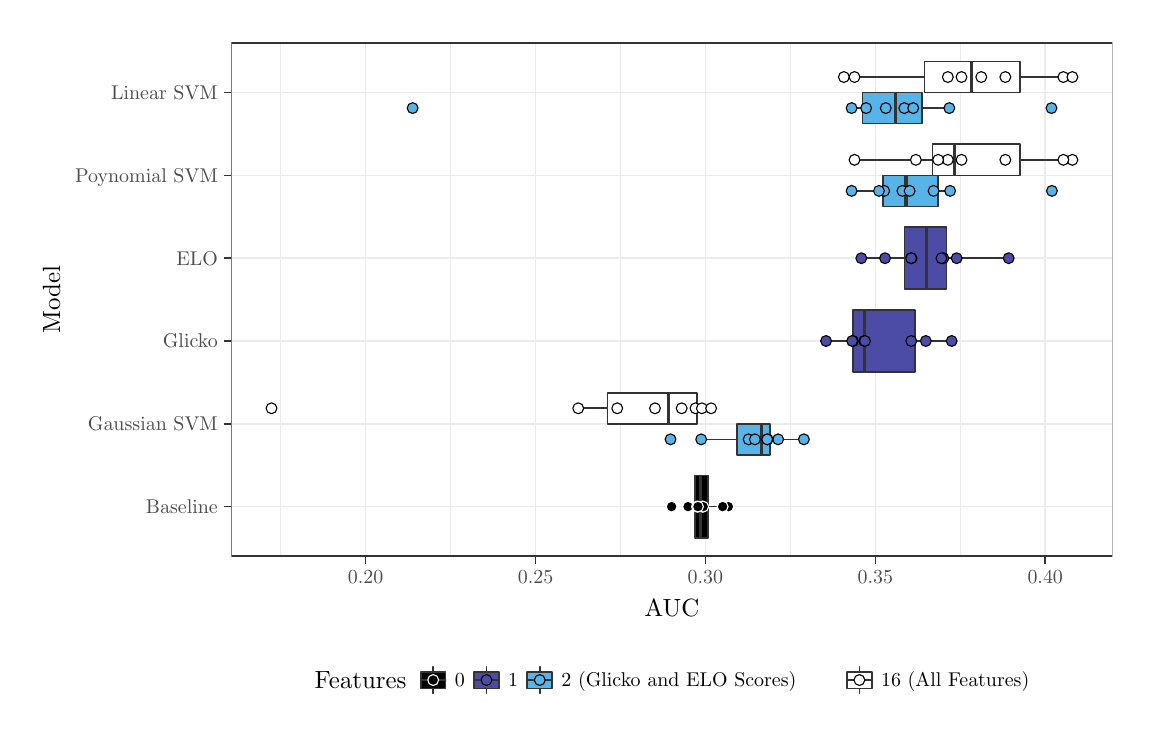
\begin{tikzpicture}[x=1pt,y=1pt]
\definecolor{fillColor}{RGB}{255,255,255}
\path[use as bounding box,fill=fillColor,fill opacity=0.00] (0,0) rectangle (397.48,252.94);
\begin{scope}
\path[clip] (  0.00,  0.00) rectangle (397.48,252.94);
\definecolor{drawColor}{RGB}{255,255,255}
\definecolor{fillColor}{RGB}{255,255,255}

\path[draw=drawColor,line width= 0.6pt,line join=round,line cap=round,fill=fillColor] (  0.00,  0.00) rectangle (397.48,252.94);
\end{scope}
\begin{scope}
\path[clip] ( 73.64, 61.91) rectangle (391.98,247.44);
\definecolor{fillColor}{RGB}{255,255,255}

\path[fill=fillColor] ( 73.64, 61.91) rectangle (391.98,247.44);
\definecolor{drawColor}{gray}{0.92}

\path[draw=drawColor,line width= 0.3pt,line join=round] ( 91.43, 61.91) --
	( 91.43,247.44);

\path[draw=drawColor,line width= 0.3pt,line join=round] (152.83, 61.91) --
	(152.83,247.44);

\path[draw=drawColor,line width= 0.3pt,line join=round] (214.22, 61.91) --
	(214.22,247.44);

\path[draw=drawColor,line width= 0.3pt,line join=round] (275.61, 61.91) --
	(275.61,247.44);

\path[draw=drawColor,line width= 0.3pt,line join=round] (337.00, 61.91) --
	(337.00,247.44);

\path[draw=drawColor,line width= 0.6pt,line join=round] ( 73.64, 79.87) --
	(391.98, 79.87);

\path[draw=drawColor,line width= 0.6pt,line join=round] ( 73.64,109.79) --
	(391.98,109.79);

\path[draw=drawColor,line width= 0.6pt,line join=round] ( 73.64,139.72) --
	(391.98,139.72);

\path[draw=drawColor,line width= 0.6pt,line join=round] ( 73.64,169.64) --
	(391.98,169.64);

\path[draw=drawColor,line width= 0.6pt,line join=round] ( 73.64,199.57) --
	(391.98,199.57);

\path[draw=drawColor,line width= 0.6pt,line join=round] ( 73.64,229.49) --
	(391.98,229.49);

\path[draw=drawColor,line width= 0.6pt,line join=round] (122.13, 61.91) --
	(122.13,247.44);

\path[draw=drawColor,line width= 0.6pt,line join=round] (183.52, 61.91) --
	(183.52,247.44);

\path[draw=drawColor,line width= 0.6pt,line join=round] (244.91, 61.91) --
	(244.91,247.44);

\path[draw=drawColor,line width= 0.6pt,line join=round] (306.31, 61.91) --
	(306.31,247.44);

\path[draw=drawColor,line width= 0.6pt,line join=round] (367.70, 61.91) --
	(367.70,247.44);
\definecolor{drawColor}{gray}{0.20}

\path[draw=drawColor,line width= 0.6pt,line join=round] (245.86, 79.87) -- (251.13, 79.87);

\path[draw=drawColor,line width= 0.6pt,line join=round] (241.04, 79.87) -- (238.62, 79.87);
\definecolor{fillColor}{RGB}{0,0,0}

\path[draw=drawColor,line width= 0.6pt,line join=round,line cap=round,fill=fillColor] (245.86, 68.65) --
	(241.04, 68.65) --
	(241.04, 91.09) --
	(245.86, 91.09) --
	(245.86, 68.65) --
	cycle;

\path[draw=drawColor,line width= 1.1pt,line join=round] (243.01, 68.65) -- (243.01, 91.09);

\path[draw=drawColor,line width= 0.6pt,line join=round] (268.32,104.18) -- (280.48,104.18);

\path[draw=drawColor,line width= 0.6pt,line join=round] (256.22,104.18) -- (243.37,104.18);
\definecolor{fillColor}{RGB}{86,180,233}

\path[draw=drawColor,line width= 0.6pt,line join=round,line cap=round,fill=fillColor] (268.32, 98.57) --
	(256.22, 98.57) --
	(256.22,109.79) --
	(268.32,109.79) --
	(268.32, 98.57) --
	cycle;

\path[draw=drawColor,line width= 1.1pt,line join=round] (265.00, 98.57) -- (265.00,109.79);

\path[draw=drawColor,line width= 0.6pt,line join=round] (241.88,115.40) -- (246.96,115.40);

\path[draw=drawColor,line width= 0.6pt,line join=round] (209.51,115.40) -- (198.94,115.40);
\definecolor{fillColor}{RGB}{255,255,255}

\path[draw=drawColor,line width= 0.6pt,line join=round,line cap=round,fill=fillColor] (241.88,109.79) --
	(209.51,109.79) --
	(209.51,121.01) --
	(241.88,121.01) --
	(241.88,109.79) --
	cycle;

\path[draw=drawColor,line width= 1.1pt,line join=round] (231.50,109.79) -- (231.50,121.01);

\path[draw=drawColor,line width= 0.6pt,line join=round] (320.60,139.72) -- (333.88,139.72);

\path[draw=drawColor,line width= 0.6pt,line join=round] (298.14,139.72) -- (288.49,139.72);
\definecolor{fillColor}{RGB}{76,76,166}

\path[draw=drawColor,line width= 0.6pt,line join=round,line cap=round,fill=fillColor] (320.60,128.50) --
	(298.14,128.50) --
	(298.14,150.94) --
	(320.60,150.94) --
	(320.60,128.50) --
	cycle;

\path[draw=drawColor,line width= 1.1pt,line join=round] (302.40,128.50) -- (302.40,150.94);

\path[draw=drawColor,line width= 0.6pt,line join=round] (332.07,169.64) -- (354.49,169.64);

\path[draw=drawColor,line width= 0.6pt,line join=round] (316.89,169.64) -- (301.23,169.64);

\path[draw=drawColor,line width= 0.6pt,line join=round,line cap=round,fill=fillColor] (332.07,158.42) --
	(316.89,158.42) --
	(316.89,180.86) --
	(332.07,180.86) --
	(332.07,158.42) --
	cycle;

\path[draw=drawColor,line width= 1.1pt,line join=round] (324.79,158.42) -- (324.79,180.86);

\path[draw=drawColor,line width= 0.6pt,line join=round] (328.84,193.96) -- (333.32,193.96);

\path[draw=drawColor,line width= 0.6pt,line join=round] (309.02,193.96) -- (297.73,193.96);
\definecolor{fillColor}{RGB}{86,180,233}

\path[draw=drawColor,line width= 0.6pt,line join=round,line cap=round,fill=fillColor] (328.84,188.34) --
	(309.02,188.34) --
	(309.02,199.57) --
	(328.84,199.57) --
	(328.84,188.34) --
	cycle;

\path[draw=drawColor,line width= 1.1pt,line join=round] (317.38,188.34) -- (317.38,199.57);

\path[draw=drawColor,line width= 0.6pt,line join=round] (358.52,205.18) -- (377.51,205.18);

\path[draw=drawColor,line width= 0.6pt,line join=round] (326.99,205.18) -- (298.78,205.18);
\definecolor{fillColor}{RGB}{255,255,255}

\path[draw=drawColor,line width= 0.6pt,line join=round,line cap=round,fill=fillColor] (358.52,199.57) --
	(326.99,199.57) --
	(326.99,210.79) --
	(358.52,210.79) --
	(358.52,199.57) --
	cycle;

\path[draw=drawColor,line width= 1.1pt,line join=round] (334.97,199.57) -- (334.97,210.79);

\path[draw=drawColor,line width= 0.6pt,line join=round] (323.25,223.88) -- (333.03,223.88);

\path[draw=drawColor,line width= 0.6pt,line join=round] (301.65,223.88) -- (297.73,223.88);
\definecolor{fillColor}{RGB}{86,180,233}

\path[draw=drawColor,line width= 0.6pt,line join=round,line cap=round,fill=fillColor] (323.25,218.27) --
	(301.65,218.27) --
	(301.65,229.49) --
	(323.25,229.49) --
	(323.25,218.27) --
	cycle;

\path[draw=drawColor,line width= 1.1pt,line join=round] (313.42,218.27) -- (313.42,229.49);

\path[draw=drawColor,line width= 0.6pt,line join=round] (358.52,235.10) -- (377.51,235.10);

\path[draw=drawColor,line width= 0.6pt,line join=round] (324.07,235.10) -- (294.94,235.10);
\definecolor{fillColor}{RGB}{255,255,255}

\path[draw=drawColor,line width= 0.6pt,line join=round,line cap=round,fill=fillColor] (358.52,229.49) --
	(324.07,229.49) --
	(324.07,240.71) --
	(358.52,240.71) --
	(358.52,229.49) --
	cycle;

\path[draw=drawColor,line width= 1.1pt,line join=round] (341.01,229.49) -- (341.01,240.71);
\definecolor{drawColor}{RGB}{255,255,255}
\definecolor{fillColor}{RGB}{0,0,0}

\path[draw=drawColor,line width= 0.4pt,line join=round,line cap=round,fill=fillColor] (232.70, 79.87) circle (  1.96);

\path[draw=drawColor,line width= 0.4pt,line join=round,line cap=round,fill=fillColor] (243.81, 79.87) circle (  1.96);

\path[draw=drawColor,line width= 0.4pt,line join=round,line cap=round,fill=fillColor] (238.62, 79.87) circle (  1.96);

\path[draw=drawColor,line width= 0.4pt,line join=round,line cap=round,fill=fillColor] (244.10, 79.87) circle (  1.96);

\path[draw=drawColor,line width= 0.4pt,line join=round,line cap=round,fill=fillColor] (241.85, 79.87) circle (  1.96);

\path[draw=drawColor,line width= 0.4pt,line join=round,line cap=round,fill=fillColor] (253.18, 79.87) circle (  1.96);

\path[draw=drawColor,line width= 0.4pt,line join=round,line cap=round,fill=fillColor] (251.13, 79.87) circle (  1.96);

\path[draw=drawColor,line width= 0.4pt,line join=round,line cap=round,fill=fillColor] (242.21, 79.87) circle (  1.96);
\definecolor{drawColor}{RGB}{0,0,0}
\definecolor{fillColor}{RGB}{255,255,255}

\path[draw=drawColor,line width= 0.4pt,line join=round,line cap=round,fill=fillColor] (241.30,115.40) circle (  1.96);

\path[draw=drawColor,line width= 0.4pt,line join=round,line cap=round,fill=fillColor] (243.61,115.40) circle (  1.96);

\path[draw=drawColor,line width= 0.4pt,line join=round,line cap=round,fill=fillColor] (236.32,115.40) circle (  1.96);

\path[draw=drawColor,line width= 0.4pt,line join=round,line cap=round,fill=fillColor] (198.94,115.40) circle (  1.96);

\path[draw=drawColor,line width= 0.4pt,line join=round,line cap=round,fill=fillColor] (213.03,115.40) circle (  1.96);

\path[draw=drawColor,line width= 0.4pt,line join=round,line cap=round,fill=fillColor] (246.96,115.40) circle (  1.96);

\path[draw=drawColor,line width= 0.4pt,line join=round,line cap=round,fill=fillColor] (226.68,115.40) circle (  1.96);

\path[draw=drawColor,line width= 0.4pt,line join=round,line cap=round,fill=fillColor] ( 88.11,115.40) circle (  1.96);
\definecolor{fillColor}{RGB}{86,180,233}

\path[draw=drawColor,line width= 0.4pt,line join=round,line cap=round,fill=fillColor] (271.18,104.18) circle (  1.96);

\path[draw=drawColor,line width= 0.4pt,line join=round,line cap=round,fill=fillColor] (280.48,104.18) circle (  1.96);

\path[draw=drawColor,line width= 0.4pt,line join=round,line cap=round,fill=fillColor] (260.51,104.18) circle (  1.96);

\path[draw=drawColor,line width= 0.4pt,line join=round,line cap=round,fill=fillColor] (262.77,104.18) circle (  1.96);

\path[draw=drawColor,line width= 0.4pt,line join=round,line cap=round,fill=fillColor] (232.29,104.18) circle (  1.96);

\path[draw=drawColor,line width= 0.4pt,line join=round,line cap=round,fill=fillColor] (267.36,104.18) circle (  1.96);

\path[draw=drawColor,line width= 0.4pt,line join=round,line cap=round,fill=fillColor] (267.23,104.18) circle (  1.96);

\path[draw=drawColor,line width= 0.4pt,line join=round,line cap=round,fill=fillColor] (243.37,104.18) circle (  1.96);
\definecolor{fillColor}{RGB}{76,76,166}

\path[draw=drawColor,line width= 0.4pt,line join=round,line cap=round,fill=fillColor] (298.21,139.72) circle (  1.96);

\path[draw=drawColor,line width= 0.4pt,line join=round,line cap=round,fill=fillColor] (302.26,139.72) circle (  1.96);

\path[draw=drawColor,line width= 0.4pt,line join=round,line cap=round,fill=fillColor] (288.49,139.72) circle (  1.96);

\path[draw=drawColor,line width= 0.4pt,line join=round,line cap=round,fill=fillColor] (333.88,139.72) circle (  1.96);

\path[draw=drawColor,line width= 0.4pt,line join=round,line cap=round,fill=fillColor] (324.55,139.72) circle (  1.96);

\path[draw=drawColor,line width= 0.4pt,line join=round,line cap=round,fill=fillColor] (297.92,139.72) circle (  1.96);

\path[draw=drawColor,line width= 0.4pt,line join=round,line cap=round,fill=fillColor] (319.29,139.72) circle (  1.96);

\path[draw=drawColor,line width= 0.4pt,line join=round,line cap=round,fill=fillColor] (302.54,139.72) circle (  1.96);

\path[draw=drawColor,line width= 0.4pt,line join=round,line cap=round,fill=fillColor] (309.81,169.64) circle (  1.96);

\path[draw=drawColor,line width= 0.4pt,line join=round,line cap=round,fill=fillColor] (330.87,169.64) circle (  1.96);

\path[draw=drawColor,line width= 0.4pt,line join=round,line cap=round,fill=fillColor] (301.23,169.64) circle (  1.96);

\path[draw=drawColor,line width= 0.4pt,line join=round,line cap=round,fill=fillColor] (319.40,169.64) circle (  1.96);

\path[draw=drawColor,line width= 0.4pt,line join=round,line cap=round,fill=fillColor] (335.69,169.64) circle (  1.96);

\path[draw=drawColor,line width= 0.4pt,line join=round,line cap=round,fill=fillColor] (330.18,169.64) circle (  1.96);

\path[draw=drawColor,line width= 0.4pt,line join=round,line cap=round,fill=fillColor] (319.24,169.64) circle (  1.96);

\path[draw=drawColor,line width= 0.4pt,line join=round,line cap=round,fill=fillColor] (354.49,169.64) circle (  1.96);
\definecolor{fillColor}{RGB}{255,255,255}

\path[draw=drawColor,line width= 0.4pt,line join=round,line cap=round,fill=fillColor] (337.44,205.18) circle (  1.96);

\path[draw=drawColor,line width= 0.4pt,line join=round,line cap=round,fill=fillColor] (298.78,205.18) circle (  1.96);

\path[draw=drawColor,line width= 0.4pt,line join=round,line cap=round,fill=fillColor] (353.28,205.18) circle (  1.96);

\path[draw=drawColor,line width= 0.4pt,line join=round,line cap=round,fill=fillColor] (332.50,205.18) circle (  1.96);

\path[draw=drawColor,line width= 0.4pt,line join=round,line cap=round,fill=fillColor] (329.00,205.18) circle (  1.96);

\path[draw=drawColor,line width= 0.4pt,line join=round,line cap=round,fill=fillColor] (377.51,205.18) circle (  1.96);

\path[draw=drawColor,line width= 0.4pt,line join=round,line cap=round,fill=fillColor] (320.95,205.18) circle (  1.96);

\path[draw=drawColor,line width= 0.4pt,line join=round,line cap=round,fill=fillColor] (374.23,205.18) circle (  1.96);
\definecolor{fillColor}{RGB}{86,180,233}

\path[draw=drawColor,line width= 0.4pt,line join=round,line cap=round,fill=fillColor] (316.08,193.96) circle (  1.96);

\path[draw=drawColor,line width= 0.4pt,line join=round,line cap=round,fill=fillColor] (309.50,193.96) circle (  1.96);

\path[draw=drawColor,line width= 0.4pt,line join=round,line cap=round,fill=fillColor] (333.32,193.96) circle (  1.96);

\path[draw=drawColor,line width= 0.4pt,line join=round,line cap=round,fill=fillColor] (370.11,193.96) circle (  1.96);

\path[draw=drawColor,line width= 0.4pt,line join=round,line cap=round,fill=fillColor] (318.69,193.96) circle (  1.96);

\path[draw=drawColor,line width= 0.4pt,line join=round,line cap=round,fill=fillColor] (297.73,193.96) circle (  1.96);

\path[draw=drawColor,line width= 0.4pt,line join=round,line cap=round,fill=fillColor] (327.35,193.96) circle (  1.96);

\path[draw=drawColor,line width= 0.4pt,line join=round,line cap=round,fill=fillColor] (307.61,193.96) circle (  1.96);
\definecolor{fillColor}{RGB}{255,255,255}

\path[draw=drawColor,line width= 0.4pt,line join=round,line cap=round,fill=fillColor] (353.28,235.10) circle (  1.96);

\path[draw=drawColor,line width= 0.4pt,line join=round,line cap=round,fill=fillColor] (294.94,235.10) circle (  1.96);

\path[draw=drawColor,line width= 0.4pt,line join=round,line cap=round,fill=fillColor] (332.50,235.10) circle (  1.96);

\path[draw=drawColor,line width= 0.4pt,line join=round,line cap=round,fill=fillColor] (298.78,235.10) circle (  1.96);

\path[draw=drawColor,line width= 0.4pt,line join=round,line cap=round,fill=fillColor] (337.44,235.10) circle (  1.96);

\path[draw=drawColor,line width= 0.4pt,line join=round,line cap=round,fill=fillColor] (344.58,235.10) circle (  1.96);

\path[draw=drawColor,line width= 0.4pt,line join=round,line cap=round,fill=fillColor] (374.23,235.10) circle (  1.96);

\path[draw=drawColor,line width= 0.4pt,line join=round,line cap=round,fill=fillColor] (377.51,235.10) circle (  1.96);
\definecolor{fillColor}{RGB}{86,180,233}

\path[draw=drawColor,line width= 0.4pt,line join=round,line cap=round,fill=fillColor] (310.07,223.88) circle (  1.96);

\path[draw=drawColor,line width= 0.4pt,line join=round,line cap=round,fill=fillColor] (333.03,223.88) circle (  1.96);

\path[draw=drawColor,line width= 0.4pt,line join=round,line cap=round,fill=fillColor] (316.77,223.88) circle (  1.96);

\path[draw=drawColor,line width= 0.4pt,line join=round,line cap=round,fill=fillColor] (139.10,223.88) circle (  1.96);

\path[draw=drawColor,line width= 0.4pt,line join=round,line cap=round,fill=fillColor] (297.73,223.88) circle (  1.96);

\path[draw=drawColor,line width= 0.4pt,line join=round,line cap=round,fill=fillColor] (302.96,223.88) circle (  1.96);

\path[draw=drawColor,line width= 0.4pt,line join=round,line cap=round,fill=fillColor] (319.98,223.88) circle (  1.96);

\path[draw=drawColor,line width= 0.4pt,line join=round,line cap=round,fill=fillColor] (369.95,223.88) circle (  1.96);
\definecolor{drawColor}{gray}{0.20}

\path[draw=drawColor,line width= 0.6pt,line join=round,line cap=round] ( 73.64, 61.91) rectangle (391.98,247.44);
\end{scope}
\begin{scope}
\path[clip] (  0.00,  0.00) rectangle (397.48,252.94);
\definecolor{drawColor}{gray}{0.30}

\node[text=drawColor,anchor=base east,inner sep=0pt, outer sep=0pt, scale=  0.72] at ( 68.69, 77.39) {Baseline};

\node[text=drawColor,anchor=base east,inner sep=0pt, outer sep=0pt, scale=  0.72] at ( 68.69,107.31) {Gaussian SVM};

\node[text=drawColor,anchor=base east,inner sep=0pt, outer sep=0pt, scale=  0.72] at ( 68.69,137.24) {Glicko};

\node[text=drawColor,anchor=base east,inner sep=0pt, outer sep=0pt, scale=  0.72] at ( 68.69,167.16) {ELO};

\node[text=drawColor,anchor=base east,inner sep=0pt, outer sep=0pt, scale=  0.72] at ( 68.69,197.09) {Poynomial SVM};

\node[text=drawColor,anchor=base east,inner sep=0pt, outer sep=0pt, scale=  0.72] at ( 68.69,227.01) {Linear SVM};
\end{scope}
\begin{scope}
\path[clip] (  0.00,  0.00) rectangle (397.48,252.94);
\definecolor{drawColor}{gray}{0.20}

\path[draw=drawColor,line width= 0.6pt,line join=round] ( 70.89, 79.87) --
	( 73.64, 79.87);

\path[draw=drawColor,line width= 0.6pt,line join=round] ( 70.89,109.79) --
	( 73.64,109.79);

\path[draw=drawColor,line width= 0.6pt,line join=round] ( 70.89,139.72) --
	( 73.64,139.72);

\path[draw=drawColor,line width= 0.6pt,line join=round] ( 70.89,169.64) --
	( 73.64,169.64);

\path[draw=drawColor,line width= 0.6pt,line join=round] ( 70.89,199.57) --
	( 73.64,199.57);

\path[draw=drawColor,line width= 0.6pt,line join=round] ( 70.89,229.49) --
	( 73.64,229.49);
\end{scope}
\begin{scope}
\path[clip] (  0.00,  0.00) rectangle (397.48,252.94);
\definecolor{drawColor}{gray}{0.20}

\path[draw=drawColor,line width= 0.6pt,line join=round] (122.13, 59.16) --
	(122.13, 61.91);

\path[draw=drawColor,line width= 0.6pt,line join=round] (183.52, 59.16) --
	(183.52, 61.91);

\path[draw=drawColor,line width= 0.6pt,line join=round] (244.91, 59.16) --
	(244.91, 61.91);

\path[draw=drawColor,line width= 0.6pt,line join=round] (306.31, 59.16) --
	(306.31, 61.91);

\path[draw=drawColor,line width= 0.6pt,line join=round] (367.70, 59.16) --
	(367.70, 61.91);
\end{scope}
\begin{scope}
\path[clip] (  0.00,  0.00) rectangle (397.48,252.94);
\definecolor{drawColor}{gray}{0.30}

\node[text=drawColor,anchor=base,inner sep=0pt, outer sep=0pt, scale=  0.72] at (122.13, 52.01) {0.20};

\node[text=drawColor,anchor=base,inner sep=0pt, outer sep=0pt, scale=  0.72] at (183.52, 52.01) {0.25};

\node[text=drawColor,anchor=base,inner sep=0pt, outer sep=0pt, scale=  0.72] at (244.91, 52.01) {0.30};

\node[text=drawColor,anchor=base,inner sep=0pt, outer sep=0pt, scale=  0.72] at (306.31, 52.01) {0.35};

\node[text=drawColor,anchor=base,inner sep=0pt, outer sep=0pt, scale=  0.72] at (367.70, 52.01) {0.40};
\end{scope}
\begin{scope}
\path[clip] (  0.00,  0.00) rectangle (397.48,252.94);
\definecolor{drawColor}{RGB}{0,0,0}

\node[text=drawColor,anchor=base,inner sep=0pt, outer sep=0pt, scale=  0.90] at (232.81, 40.31) {AUC};
\end{scope}
\begin{scope}
\path[clip] (  0.00,  0.00) rectangle (397.48,252.94);
\definecolor{drawColor}{RGB}{0,0,0}

\node[text=drawColor,rotate= 90.00,anchor=base,inner sep=0pt, outer sep=0pt, scale=  0.90] at ( 11.70,154.68) {Model};
\end{scope}
\begin{scope}
\path[clip] (  0.00,  0.00) rectangle (397.48,252.94);
\definecolor{fillColor}{RGB}{255,255,255}

\path[fill=fillColor] ( 98.01,  5.50) rectangle (367.61, 28.93);
\end{scope}
\begin{scope}
\path[clip] (  0.00,  0.00) rectangle (397.48,252.94);
\definecolor{drawColor}{RGB}{0,0,0}

\node[text=drawColor,anchor=base west,inner sep=0pt, outer sep=0pt, scale=  0.90] at (103.70, 14.11) {Features};
\end{scope}
\begin{scope}
\path[clip] (  0.00,  0.00) rectangle (397.48,252.94);
\definecolor{fillColor}{RGB}{255,255,255}

\path[fill=fillColor] (140.50, 11.19) rectangle (152.55, 23.24);
\end{scope}
\begin{scope}
\path[clip] (  0.00,  0.00) rectangle (397.48,252.94);
\definecolor{drawColor}{gray}{0.20}

\path[draw=drawColor,line width= 0.6pt,line join=round,line cap=round] (146.53, 12.40) --
	(146.53, 14.20);

\path[draw=drawColor,line width= 0.6pt,line join=round,line cap=round] (146.53, 20.22) --
	(146.53, 22.03);
\definecolor{fillColor}{RGB}{0,0,0}

\path[draw=drawColor,line width= 0.6pt,line join=round,line cap=round,fill=fillColor] (142.01, 14.20) rectangle (151.04, 20.22);

\path[draw=drawColor,line width= 0.6pt,line join=round,line cap=round] (142.01, 17.21) --
	(151.04, 17.21);
\end{scope}
\begin{scope}
\path[clip] (  0.00,  0.00) rectangle (397.48,252.94);
\definecolor{drawColor}{RGB}{255,255,255}
\definecolor{fillColor}{RGB}{0,0,0}

\path[draw=drawColor,line width= 0.4pt,line join=round,line cap=round,fill=fillColor] (146.53, 17.21) circle (  1.96);
\end{scope}
\begin{scope}
\path[clip] (  0.00,  0.00) rectangle (397.48,252.94);
\definecolor{fillColor}{RGB}{255,255,255}

\path[fill=fillColor] (159.76, 11.19) rectangle (171.81, 23.24);
\end{scope}
\begin{scope}
\path[clip] (  0.00,  0.00) rectangle (397.48,252.94);
\definecolor{drawColor}{gray}{0.20}

\path[draw=drawColor,line width= 0.6pt,line join=round,line cap=round] (165.78, 12.40) --
	(165.78, 14.20);

\path[draw=drawColor,line width= 0.6pt,line join=round,line cap=round] (165.78, 20.22) --
	(165.78, 22.03);
\definecolor{fillColor}{RGB}{76,76,166}

\path[draw=drawColor,line width= 0.6pt,line join=round,line cap=round,fill=fillColor] (161.27, 14.20) rectangle (170.30, 20.22);

\path[draw=drawColor,line width= 0.6pt,line join=round,line cap=round] (161.27, 17.21) --
	(170.30, 17.21);
\end{scope}
\begin{scope}
\path[clip] (  0.00,  0.00) rectangle (397.48,252.94);
\definecolor{drawColor}{RGB}{0,0,0}
\definecolor{fillColor}{RGB}{76,76,166}

\path[draw=drawColor,line width= 0.4pt,line join=round,line cap=round,fill=fillColor] (165.78, 17.21) circle (  1.96);
\end{scope}
\begin{scope}
\path[clip] (  0.00,  0.00) rectangle (397.48,252.94);
\definecolor{fillColor}{RGB}{255,255,255}

\path[fill=fillColor] (179.02, 11.19) rectangle (191.06, 23.24);
\end{scope}
\begin{scope}
\path[clip] (  0.00,  0.00) rectangle (397.48,252.94);
\definecolor{drawColor}{gray}{0.20}

\path[draw=drawColor,line width= 0.6pt,line join=round,line cap=round] (185.04, 12.40) --
	(185.04, 14.20);

\path[draw=drawColor,line width= 0.6pt,line join=round,line cap=round] (185.04, 20.22) --
	(185.04, 22.03);
\definecolor{fillColor}{RGB}{86,180,233}

\path[draw=drawColor,line width= 0.6pt,line join=round,line cap=round,fill=fillColor] (180.52, 14.20) rectangle (189.56, 20.22);

\path[draw=drawColor,line width= 0.6pt,line join=round,line cap=round] (180.52, 17.21) --
	(189.56, 17.21);
\end{scope}
\begin{scope}
\path[clip] (  0.00,  0.00) rectangle (397.48,252.94);
\definecolor{drawColor}{RGB}{0,0,0}
\definecolor{fillColor}{RGB}{86,180,233}

\path[draw=drawColor,line width= 0.4pt,line join=round,line cap=round,fill=fillColor] (185.04, 17.21) circle (  1.96);
\end{scope}
\begin{scope}
\path[clip] (  0.00,  0.00) rectangle (397.48,252.94);
\definecolor{fillColor}{RGB}{255,255,255}

\path[fill=fillColor] (294.52, 11.19) rectangle (306.57, 23.24);
\end{scope}
\begin{scope}
\path[clip] (  0.00,  0.00) rectangle (397.48,252.94);
\definecolor{drawColor}{gray}{0.20}

\path[draw=drawColor,line width= 0.6pt,line join=round,line cap=round] (300.55, 12.40) --
	(300.55, 14.20);

\path[draw=drawColor,line width= 0.6pt,line join=round,line cap=round] (300.55, 20.22) --
	(300.55, 22.03);
\definecolor{fillColor}{RGB}{255,255,255}

\path[draw=drawColor,line width= 0.6pt,line join=round,line cap=round,fill=fillColor] (296.03, 14.20) rectangle (305.06, 20.22);

\path[draw=drawColor,line width= 0.6pt,line join=round,line cap=round] (296.03, 17.21) --
	(305.06, 17.21);
\end{scope}
\begin{scope}
\path[clip] (  0.00,  0.00) rectangle (397.48,252.94);
\definecolor{drawColor}{RGB}{0,0,0}
\definecolor{fillColor}{RGB}{255,255,255}

\path[draw=drawColor,line width= 0.4pt,line join=round,line cap=round,fill=fillColor] (300.55, 17.21) circle (  1.96);
\end{scope}
\begin{scope}
\path[clip] (  0.00,  0.00) rectangle (397.48,252.94);
\definecolor{drawColor}{RGB}{0,0,0}

\node[text=drawColor,anchor=base west,inner sep=0pt, outer sep=0pt, scale=  0.72] at (154.36, 14.73) {0};
\end{scope}
\begin{scope}
\path[clip] (  0.00,  0.00) rectangle (397.48,252.94);
\definecolor{drawColor}{RGB}{0,0,0}

\node[text=drawColor,anchor=base west,inner sep=0pt, outer sep=0pt, scale=  0.72] at (173.61, 14.73) {1};
\end{scope}
\begin{scope}
\path[clip] (  0.00,  0.00) rectangle (397.48,252.94);
\definecolor{drawColor}{RGB}{0,0,0}

\node[text=drawColor,anchor=base west,inner sep=0pt, outer sep=0pt, scale=  0.72] at (192.87, 14.73) {2 (Glicko and ELO Scores)};
\end{scope}
\begin{scope}
\path[clip] (  0.00,  0.00) rectangle (397.48,252.94);
\definecolor{drawColor}{RGB}{0,0,0}

\node[text=drawColor,anchor=base west,inner sep=0pt, outer sep=0pt, scale=  0.72] at (308.38, 14.73) {16 (All Features)};
\end{scope}
\end{tikzpicture}
